\chapter{注意力和动作的视觉处理} \label{chap:chap25}

人脑具有惊人的能力,可以将动作指向视觉世界中的物体——婴儿伸手去拿物体,网球运动员击球,艺术家看着模特。
这种能力需要视觉系统解决三个问题:
对视觉世界进行空间精确分析,从视觉世界的混乱刺激中选择感兴趣的物体,并将物体的位置和细节信息传递给电机系统。



\section{大脑补偿眼球运动以创建视觉世界的稳定表示}

尽管视觉系统可以生动地再现我们的视觉世界,如前几章所述,但视觉图像不像瞬时照片记录,而是根据眼睛的几个离散神经通路传递的信息动态构建的。
例如,当我们看一幅画时,我们会通过一系列快速的眼球运动(扫视)来探索它,这些运动会将中央凹重新定向到视野中感兴趣的不同物体。
在从视网膜中的光刺激产生可解释的视觉图像的过程中,大脑必须考虑到这些眼球运动。


当每个扫视将一个新物体带到中央凹时,整个视觉世界的图像都会在中央凹上发生变化。
这些变化每秒发生几次,以至于几分钟后运动记录变得混乱(图~\ref{fig:25_1})。
通过这种不断的移动,视觉图像应该类似于业余视频,其中图像会四处晃动,因为摄像师不熟练地保持相机稳定。 
然而,事实上,我们的视力是如此稳定,以至于我们通常不会意识到眼跳的视觉效果。
之所以如此,是因为大脑在每次扫视后都会对落在视网膜上的图像进行持续调整。


\begin{figure}[htbp]
	\centering
	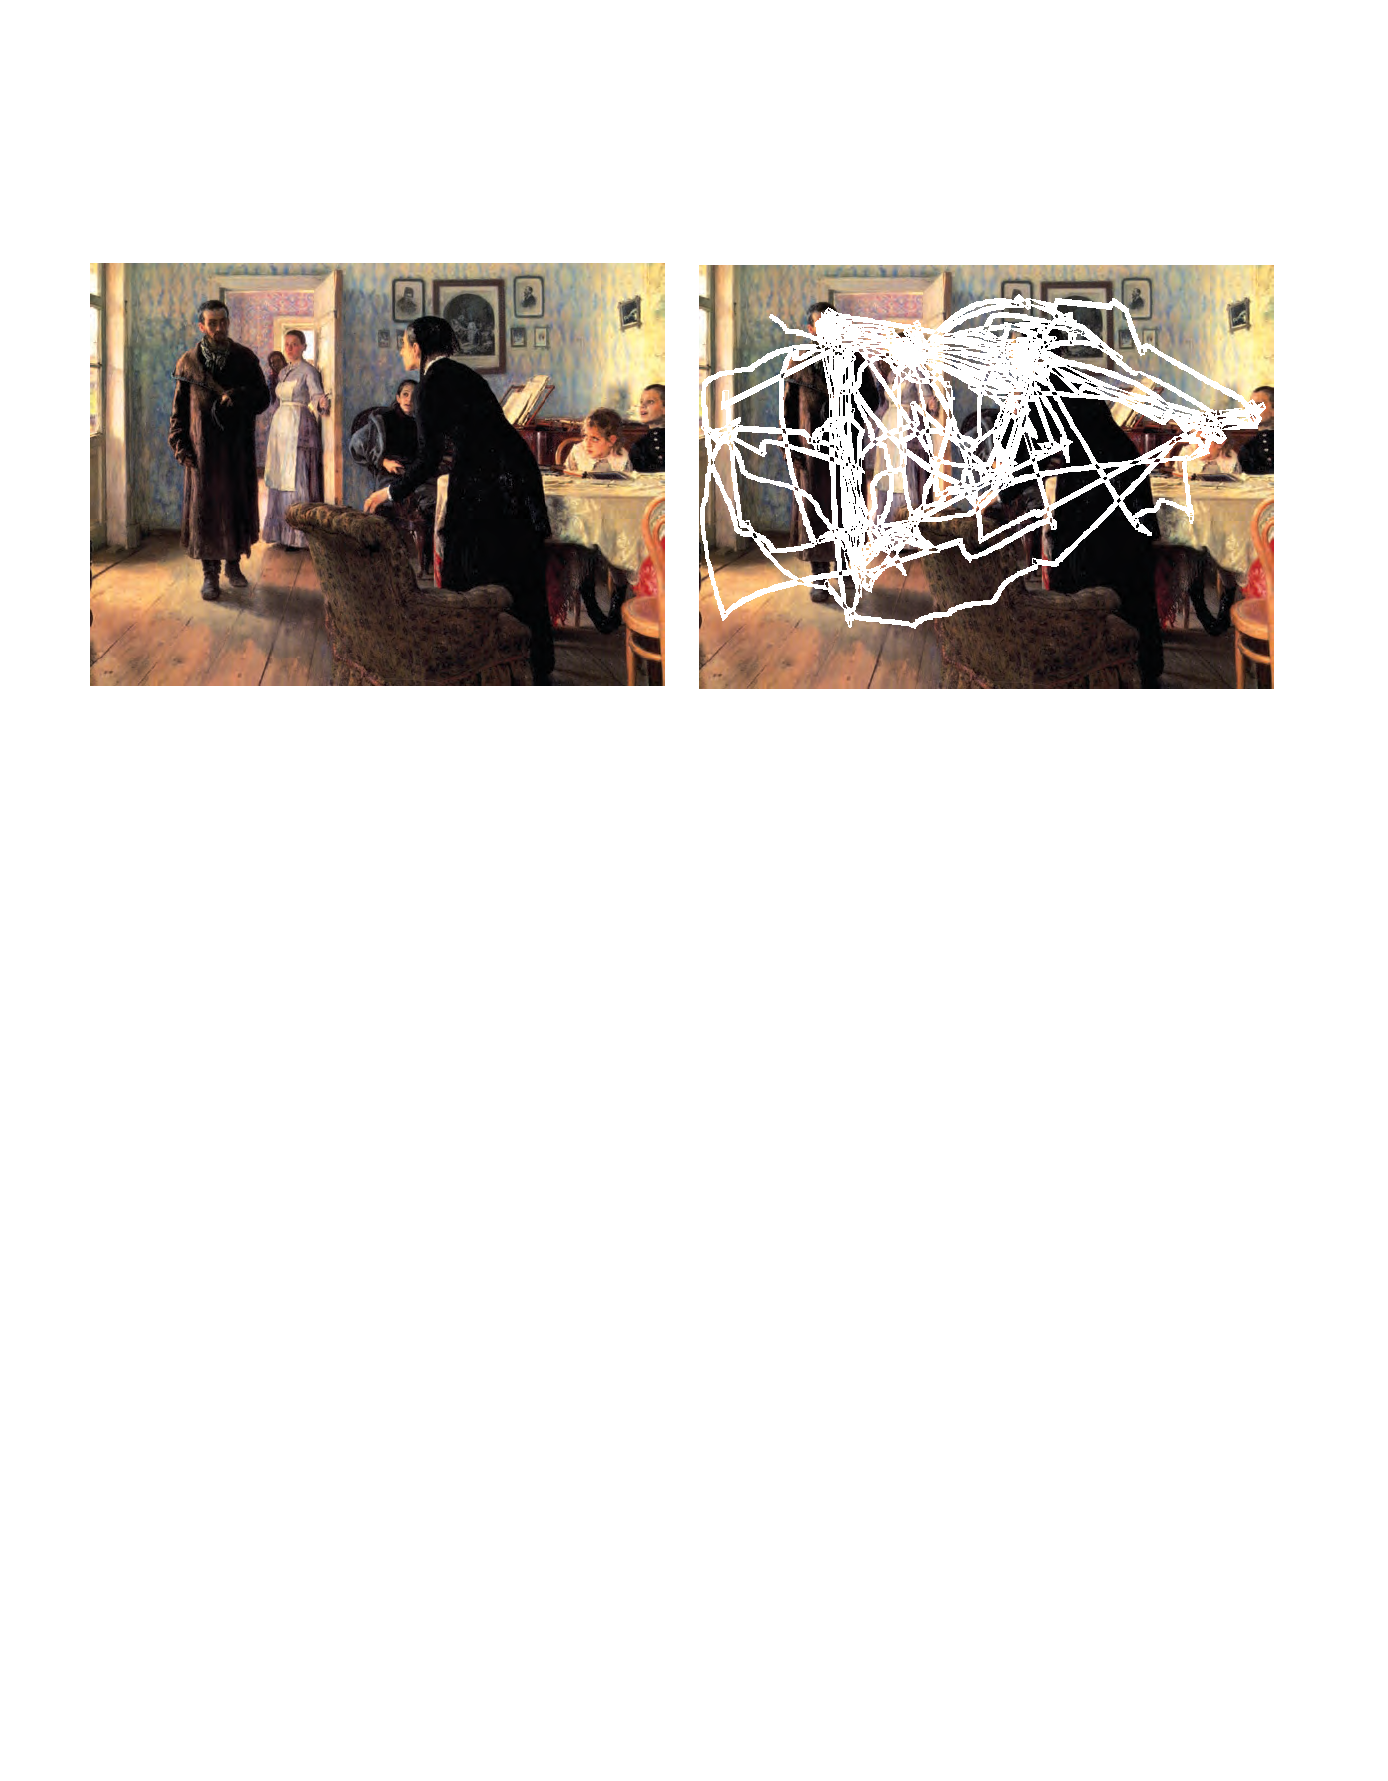
\includegraphics[width=0.65\linewidth]{chap25/fig_25_1}
	\caption{视觉过程中的眼球运动。受试者观看这幅画(llya Repin 的《意外访客》)几分钟,对选定的注视点进行扫视,主要是面部。 线条表示扫视,斑点表示注视点。 (经许可转载自 Yarbus 1967)。}
	\label{fig:25_1}
\end{figure}


如图~\ref{fig:25_2}~所示,一个简单的实验室实验说明了大脑面临的生物学挑战。


\begin{figure}[htbp]
	\centering
	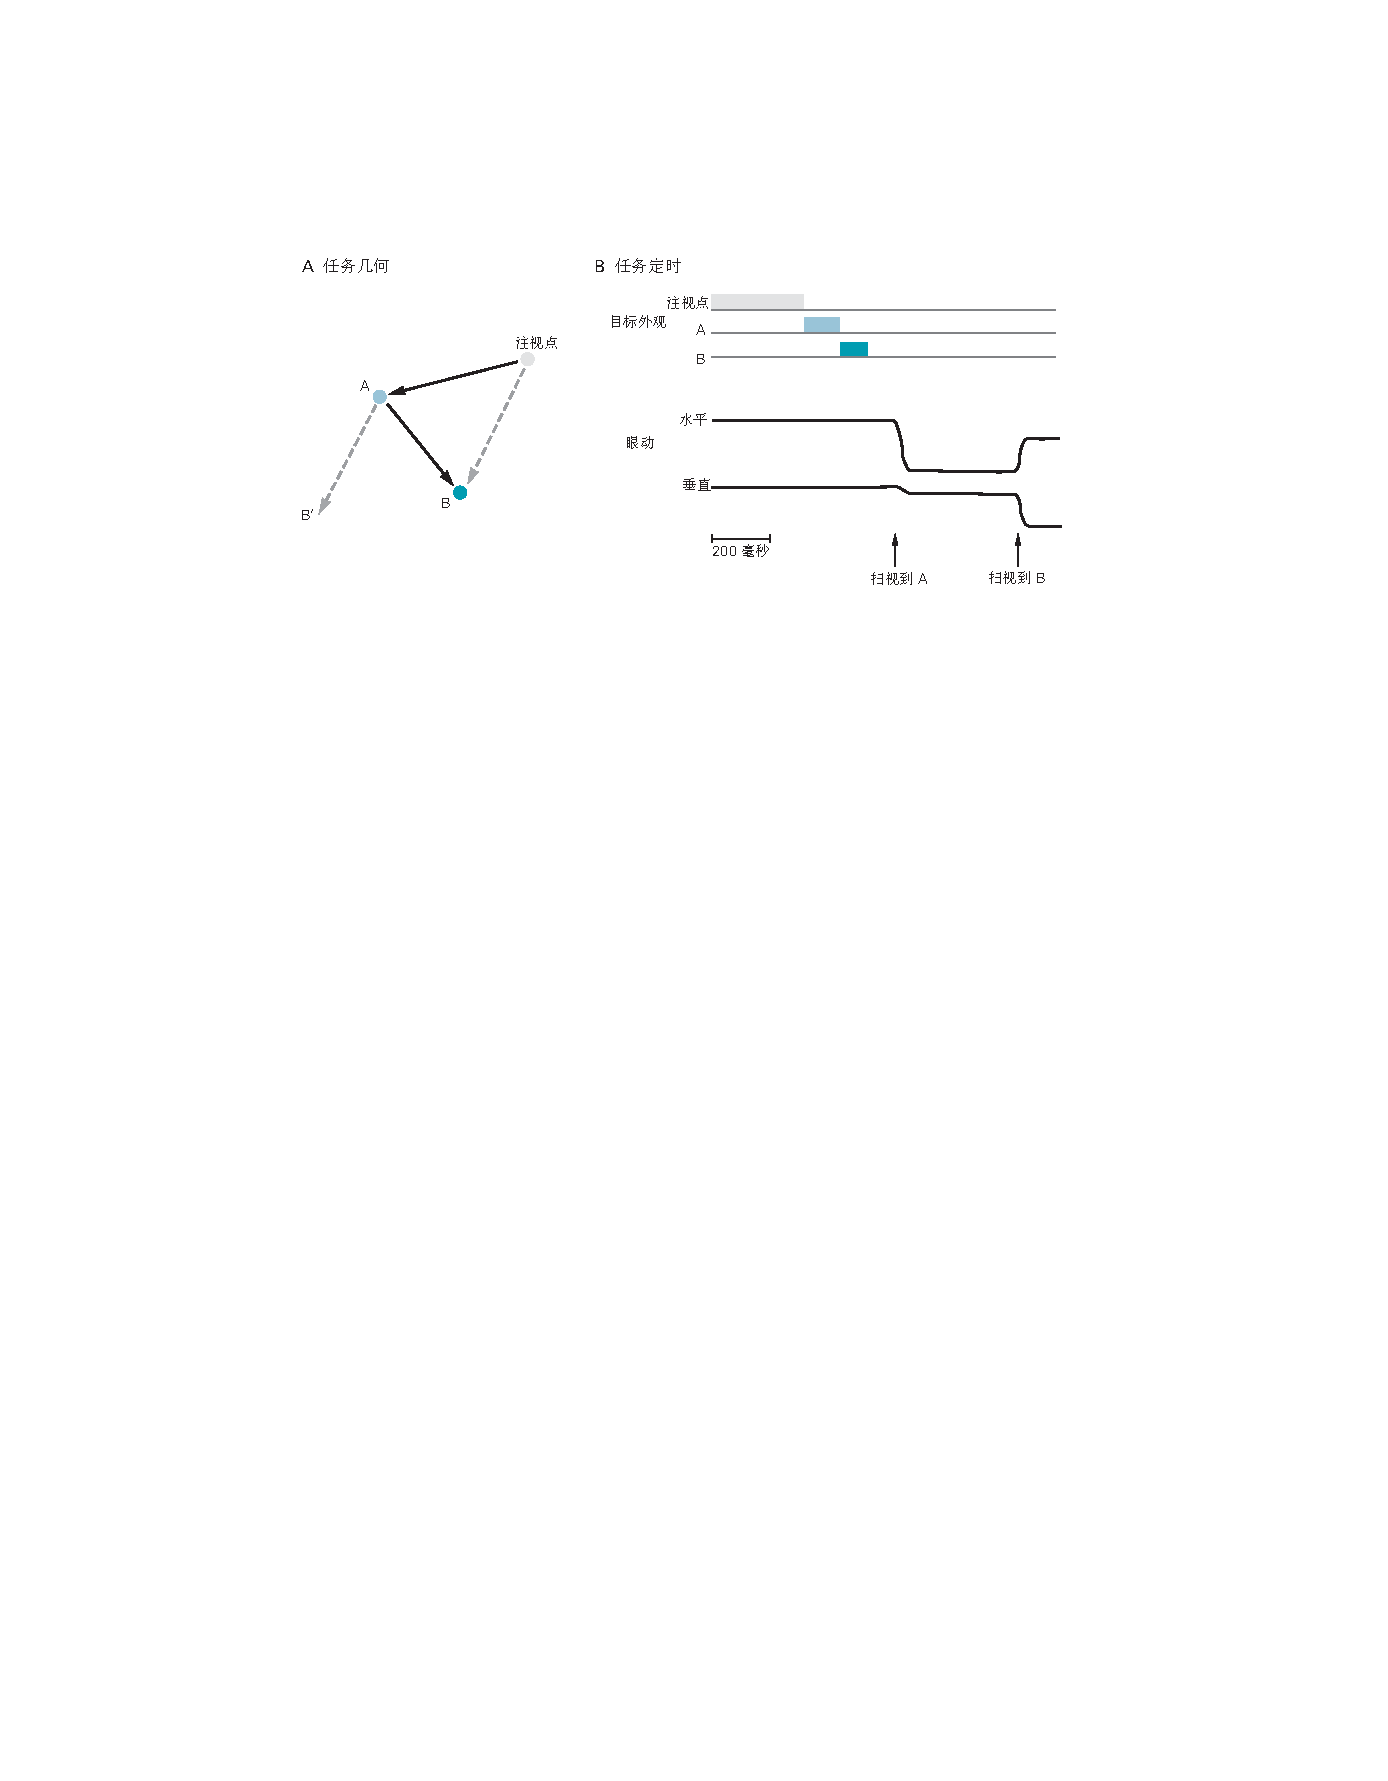
\includegraphics[width=0.75\linewidth]{chap25/fig_25_2}
	\caption{双步任务说明大脑如何在扫视期间稳定图像。 A. 受试者首先注视一个消失的注视点 (FP),然后两个扫视目标 A 和 B 依次出现和消失,然后受试者才能进行扫视。 第一个扫视(目标 A)很简单。 视网膜矢量 (FP→A) 和眼跳矢量相同。 第一次扫视后,被试正在看A,视网膜向量为A→B',但猴子必须进行一次扫视,向量为A→B。 大脑必须调整视网膜矢量以补偿第一个扫视。 B. 时机。 上面的记录显示目标出现的时间(彩色条)。 (缩写:H,水平;V,垂直。)}
	\label{fig:25_2}
\end{figure}



\subsection{扫视的运动指令被复制到视觉系统}

对视觉稳定性背后的大脑机制的第一个洞察来自 Hermann von Helmholtz 在 19 世纪的观察。
他看到一名患者由于外直肌麻痹而无法将眼睛水平地移向耳朵。
每当患者试图看向他的耳朵时,整个视觉世界就会跳向相反的方向,然后回到注视的中心。


Helmholtz 假设每个扫视的运动命令副本被馈送到视觉系统,以便可以调整视觉世界的表示以补偿眼球运动。
这种调整将导致视觉世界的稳定图像。
在 19 世纪,亥姆霍兹称这样的副本为“努力感”,而在 20 世纪,它被命名为输出副本或推论放电。


推论放电解决了双步扫视的问题。
为了使必然放电影响眼球运动的视觉感知,运动信息必须影响视觉神经元的活动。
当猴子进行扫视时,顶叶皮层、额叶眼区、纹状体视觉皮层和上丘中的神经元就会发生这种情况。
每个眼跳都可以被认为是一个具有两个维度的向量——方向和振幅。
尽管每次扫视后的视网膜图像都不同,但大脑可以使用每次扫视的向量从视网膜图像序列中重建整个视觉场景。


可以在单个电池的水平上看到推论放电。
对恒河猴(一种动眼神经和视觉系统类似于人类的动物)的生理学研究阐明了这个问题。
每次猴子进行扫视时,当前不在外侧顶内区域神经元的感受野中的刺激,因此无法激发神经元,如果即将发生的扫视将刺激带入感受野,则会激发神经元, 甚至在扫视发生之前(图~\ref{fig:25_3})。
因此,即将发生的眼跳的必然放电会影响顶叶神经元的视觉反应。


\begin{figure}[htbp]
	\centering
	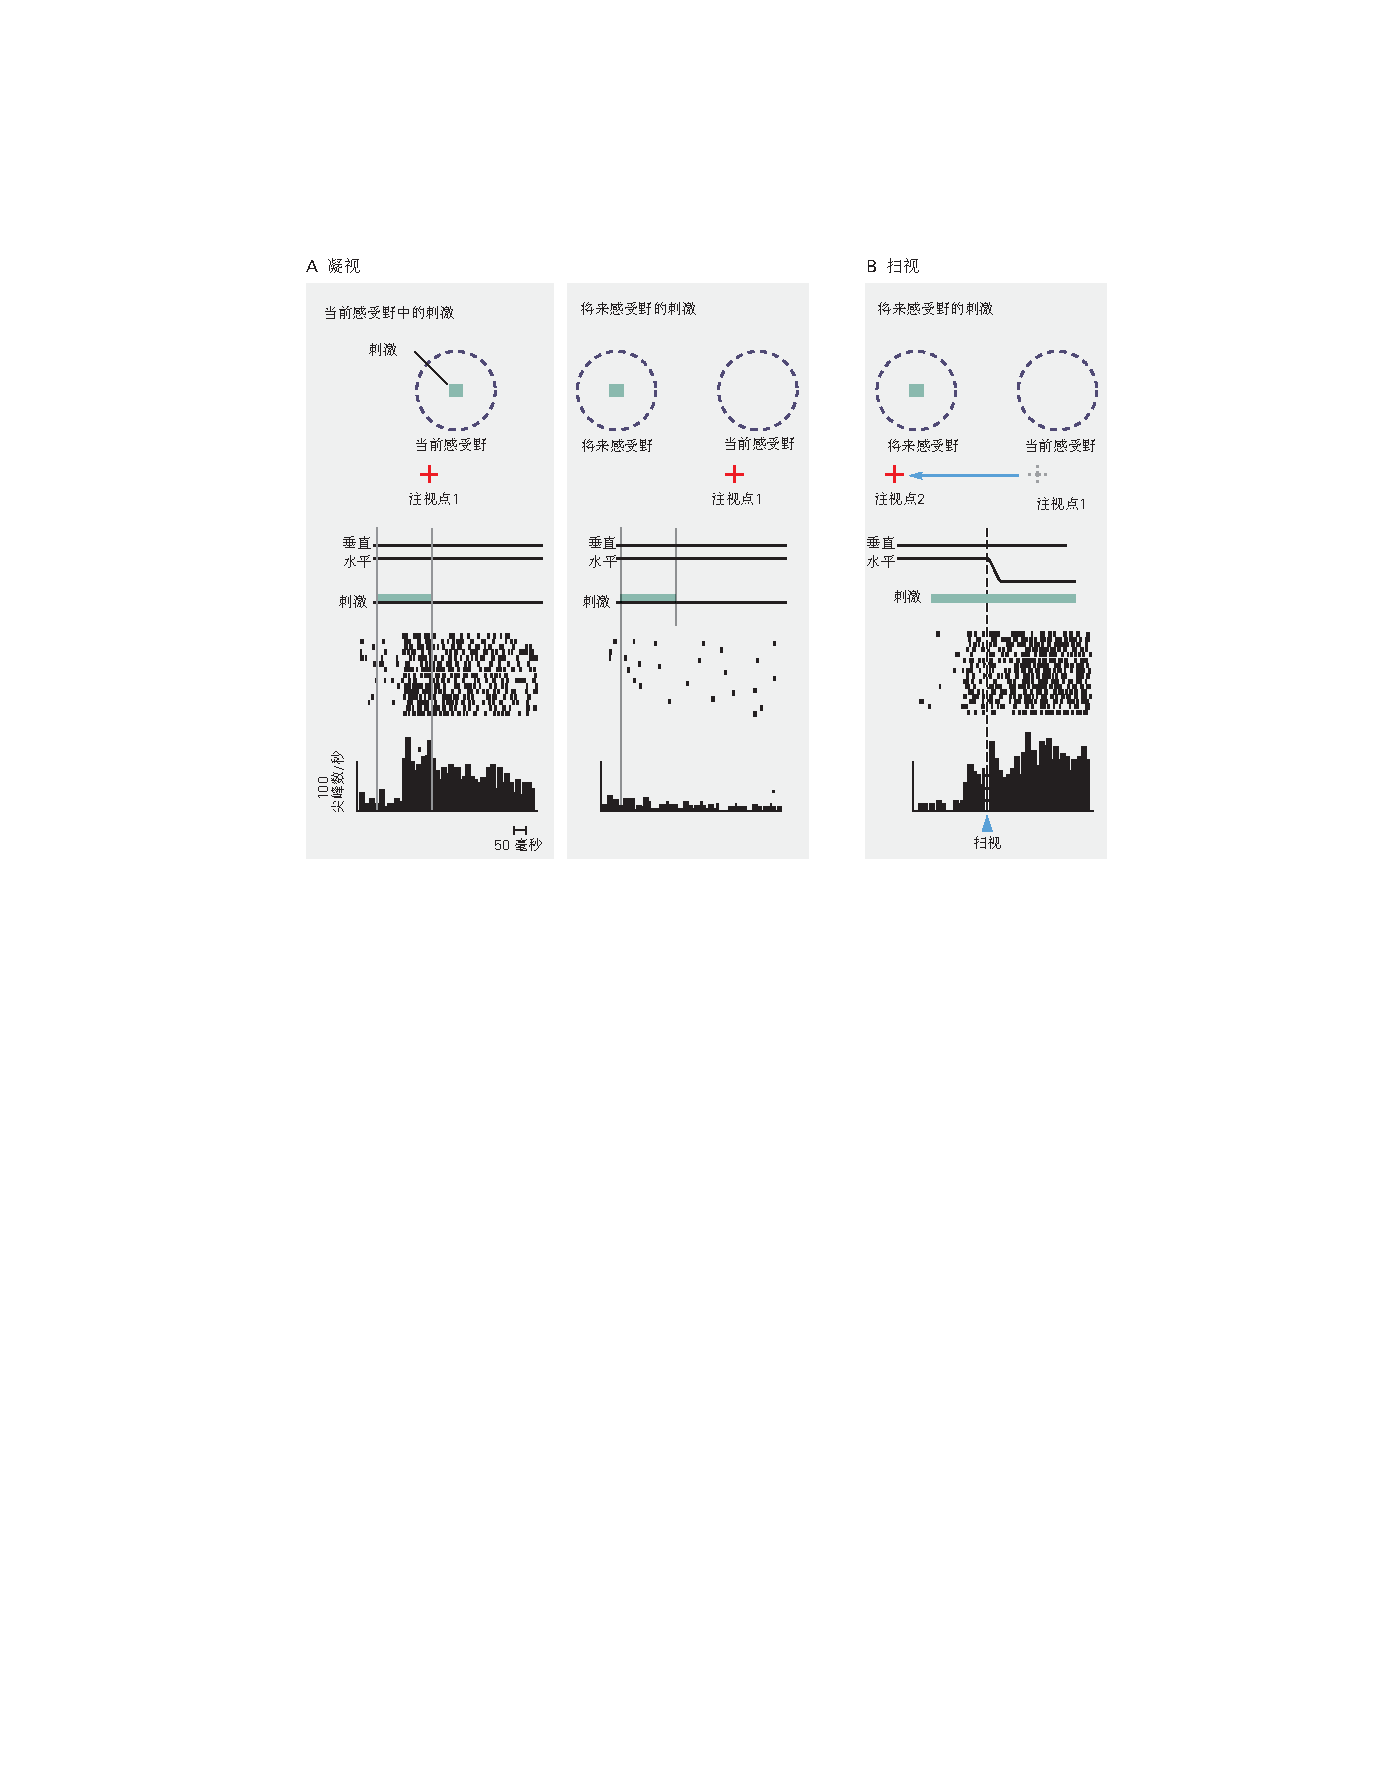
\includegraphics[width=0.75\linewidth]{chap25/fig_25_3}
	\caption{重新映射猴子顶叶皮层视觉神经元的感受野与扫视眼球运动。(A [左] 和 B 经许可改编自 Duhamel、Colby 和 Goldberg 1992。A [右] 经许可转载自 M.E. Goldberg。)A. 左:猴子注视注视点 1 (FP1),并且 细胞对当前感受野 (CRF) 中突然出现的与任务无关的刺激做出反应。 连续试验在刺激出现时同步。 (缩写:H,水平眼位;V,垂直眼位。)右图:猴子看着 FP1,细胞对未来感受野 (FRF) 中闪现的刺激没有反应。B. 猴子从 FP1 到 FP2 进行扫视,这会将细胞的感受野带到 FRF 中的刺激上。现在细胞甚至在眼跳开始之前就开始放电,这意味着眼跳计划的必然放电重新映射了细胞响应的视网膜区域。}
	\label{fig:25_3}
\end{figure}


这种感受野的瞬态重新映射解释了受试者如何执行双步任务。
考虑图 25–2A 中的图表。
任务从猴子将目光对准注视点 (FP) 开始。
在猴子进行第一次扫视后,视网膜矢量 A→B' 不再对进行 A→B 扫视有用。
然而,FP→A 扫视重新映射描述向量 A→B 的细胞活动,因此它对 B 视网膜位置的目标做出反应,当猴子看 FP 时,该位置不在其感受野内。
在许多皮层和皮层下区域发现重映射,包括外侧顶内区、额叶视野、内侧顶内区、上丘中间层和前纹状体区 V4、V3a 和 V2。
正如我们将看到的,重新映射有助于围绕扫视时间的视觉感知和视觉引导运动的准确性。


这提出的第一个问题是:大脑如何获得它反馈给视觉系统的扫视向量?
我们从数十年的研究中了解到,矢量的运动指令在中脑顶部的上丘中得到体现(第~\ref{chap:chap35}~章)。
上丘中的每个神经元都被调整到给定向量的眼跳,这样神经元共同提供所有可能眼跳的向量图。
上丘的失活会影响猴子进行眼跳的能力。
上丘的电刺激会引起刺激部位神经元所描述的矢量眼跳。 
但这提供了实际驱动眼睛的向量,而不是通知关于扫视向量的感知的向量。
用于移动眼睛的矢量信息如何可用于不移动眼睛但需要有关其移动方式的信息的大脑过程?


由于在上丘中已经确定了移动眼睛的矢量,因此可以合理地预期这也可能是必然放电的来源。
它的确是。
上丘既有产生眼跳的下行通路,也有通往大脑皮层的上行通路,可以携带即将发生的运动的必然放电(图 25-4)。
到达大脑皮层的通路通过丘脑,所有内部信息和几乎所有外部信息都通过丘脑到达大脑皮层。


\begin{figure}[htbp]
	\centering
	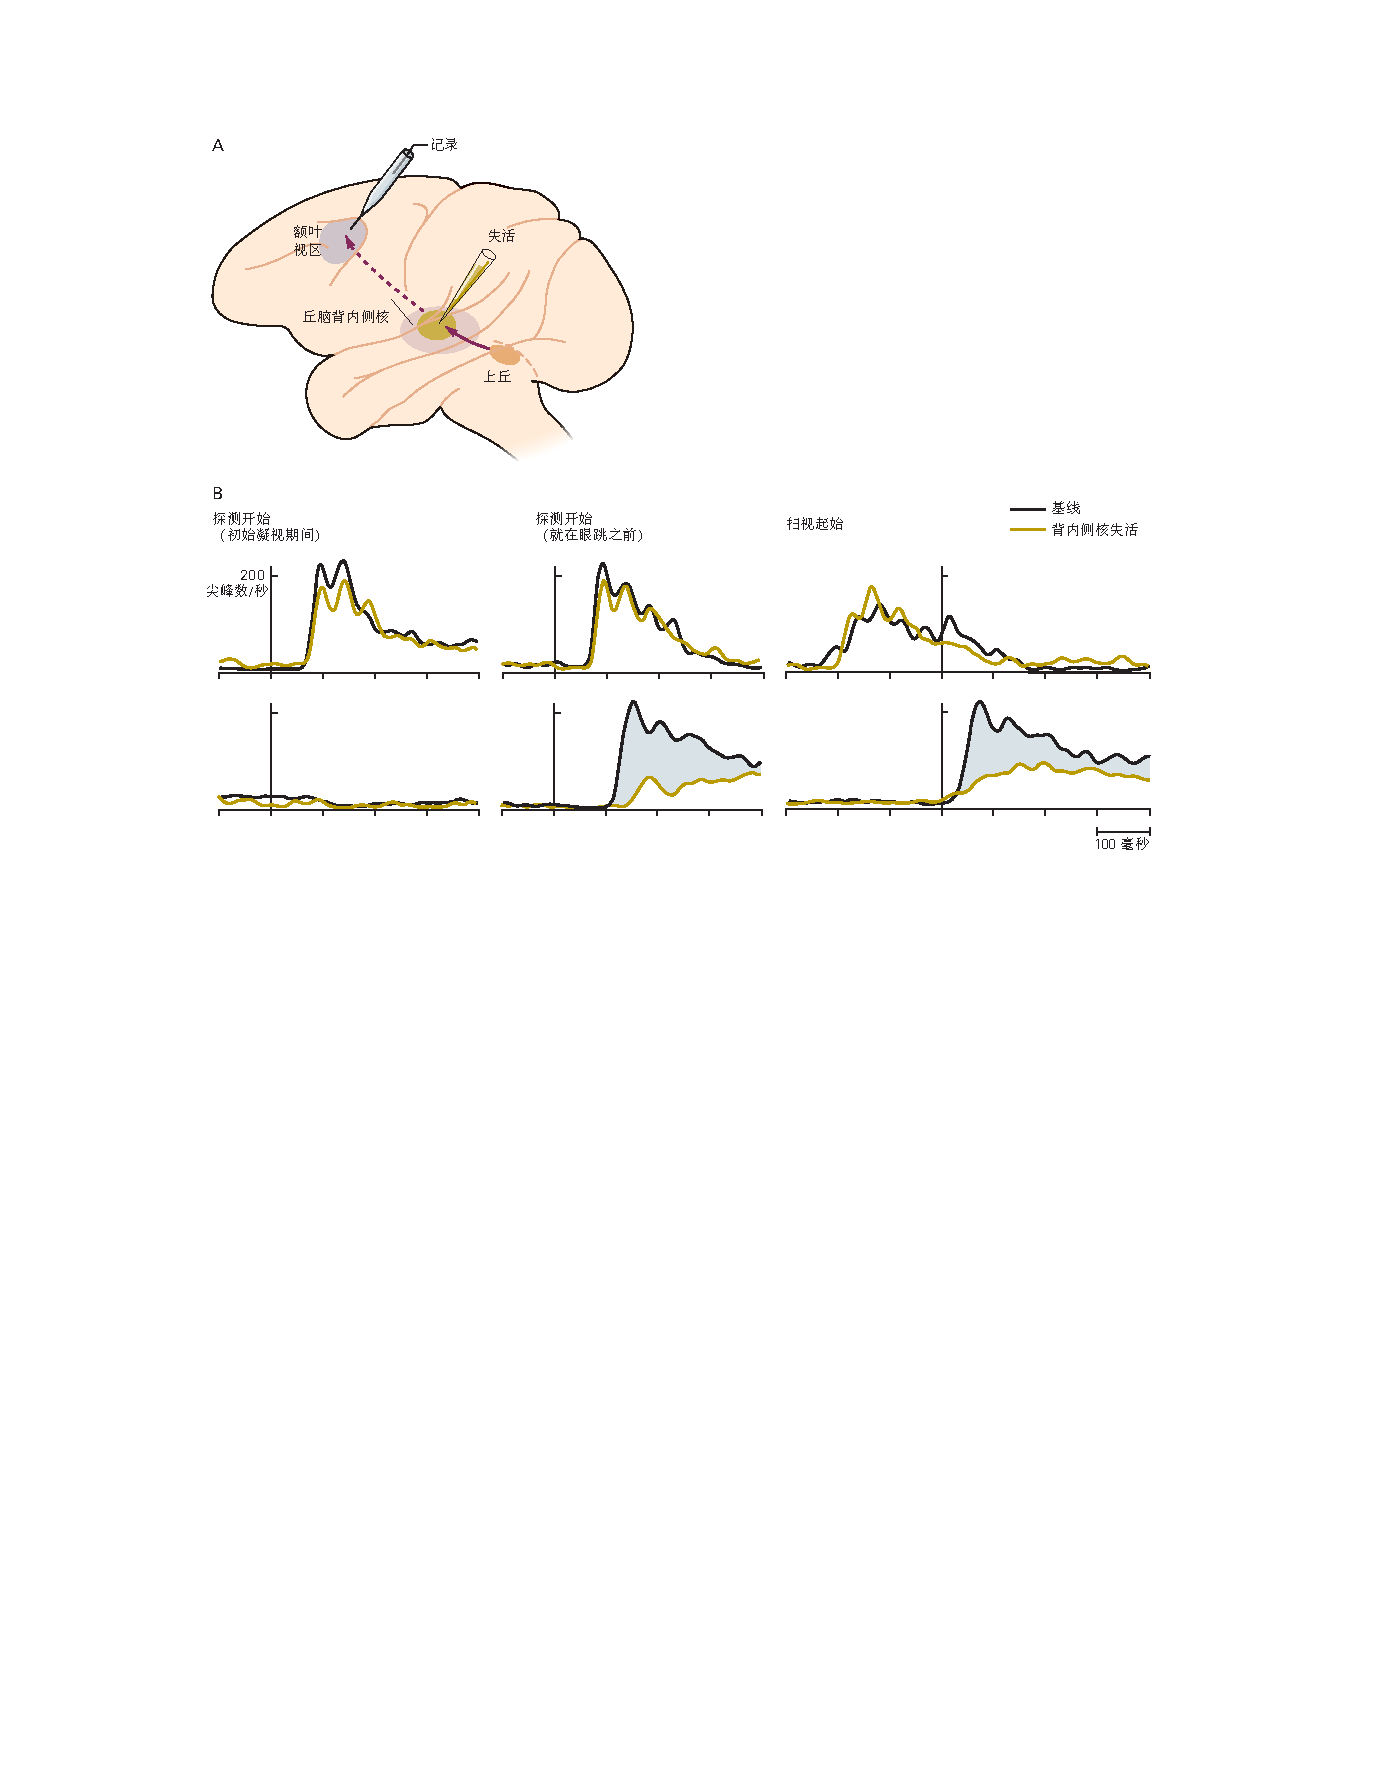
\includegraphics[width=0.8\linewidth]{chap25/fig_25_4}
	\caption{扫视运动程序的必然放电会导致在扫视之前额叶眼场神经元的感受野位置发生变化。(经许可改编自 Sommer 和 Wurtz 2008。Annual Reviews 版权所有 © 2008。)A. 必然放电的一种可能途径起源于上丘中产生眼跳的神经元,穿过丘脑的内侧背核, 并终止于额叶皮质的额叶眼区 (FEF)。B. 当内侧背核 (MD) 失活时,额眼场神经元对细胞当前感受野中刺激探针的反应不受影响(上部记录),而对未来刺激的反应(后- 扫视)感受野严重受损(记录较低)。 这一结果表明,扫视运动程序的必然放电指导神经元感受野特性的转变。}
	\label{fig:25_4}
\end{figure}


丘脑中的运动信号不一定是必然放电;
它也可能是简单地通过大脑皮层的运动命令。
然而,情况并非如此,因为丘脑中这条通路的失活不会改变眼跳的幅度和方向。
它不是在驱动扫视。
它更有可能是必然激活。
丘脑通路失活后,猴子无法准确执行双步任务的第二次扫视。
此外,失活会破坏前面描述的感受野重新映射(图 ~\ref{fig:25_3}B)。
因为破坏推论放电会破坏感受野重新映射和眼球运动的行为补偿,推论放电可能对于解决动作的空间准确性问题至关重要。


为了确定推论放电是否也提供了允许视觉系统感知在扫视之前出现的物体位置的信息,猴子被训练以指示它认为它的眼睛在扫视结束时指向的位置。
我们可以测量运动系统移动眼睛的位置,但我们想知道的是猴子对每次扫视时眼睛方向变化的感知。
这可以使用 Heiner Deubel 及其同事为人类开发并适用于猴子的任务来确定。
在此任务中,猴子注视一个注视点,然后扫视一个目标(图~\ref{fig:25_5}A)。
在扫视过程中,目标暂时消失;
当它再次出现时,它已被移至原始目标的左侧或右侧位置。
试验后,猴子向右或向左移动一个条以指示位移的方向(图~\ref{fig:25_5}A)。


\begin{figure}[htbp]
	\centering
	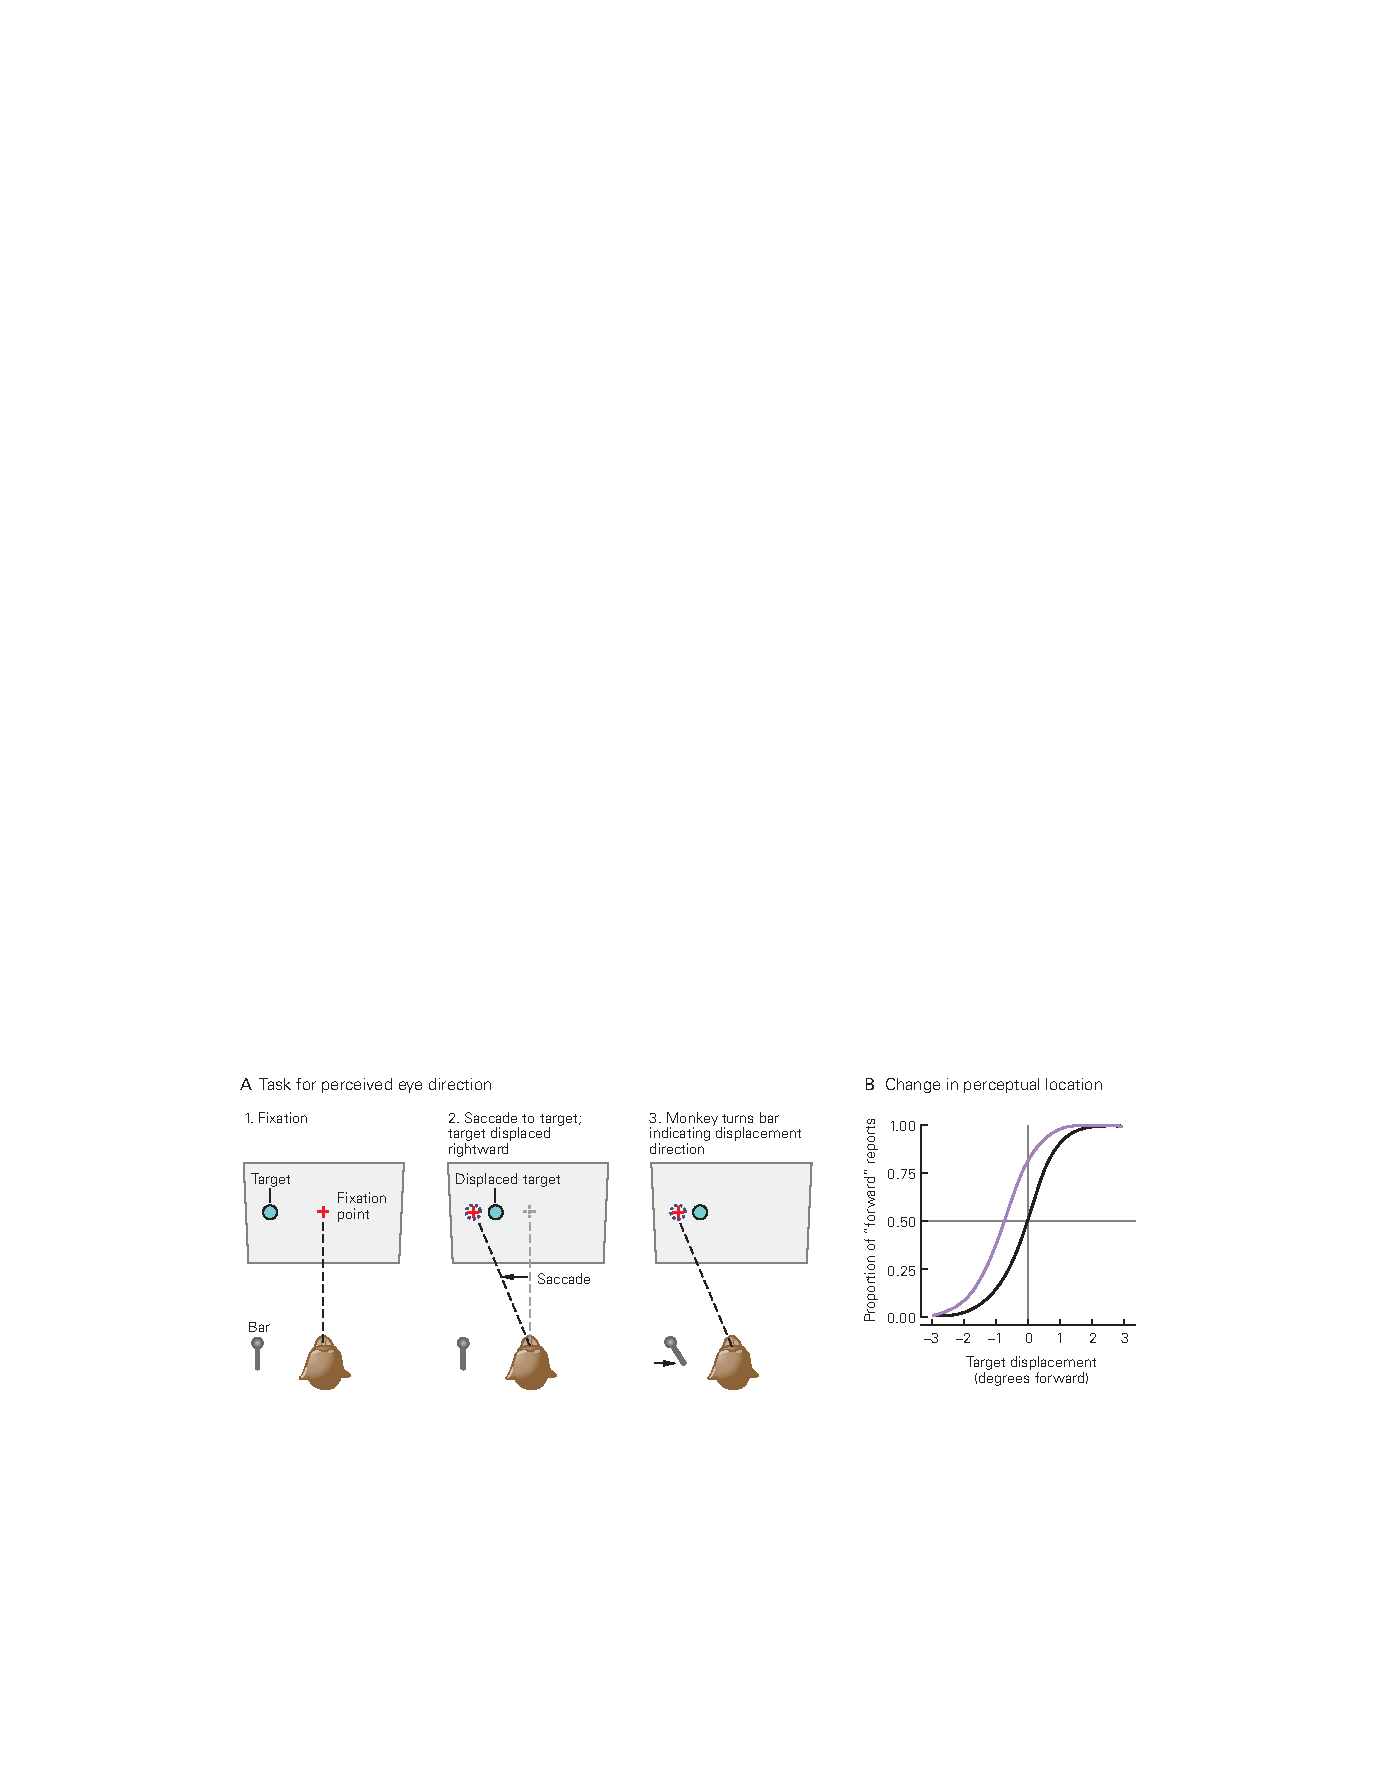
\includegraphics[width=0.8\linewidth]{chap25/fig_25_5}
	\caption{感知到的扫视方向随着必然放电的中断而改变。 A. 在每次试验开始时,猴子都会在屏幕上注视一个目标 (1)。 当注视点关闭时,猴子会向目标扫视; 在扫视期间,目标随机(最多 3°)向左或向右移动 (2)。 在扫视到原始目标后,猴子会收到一个奖励,用于在目标位移 (3) 的方向上手动移动一个杆。 B. 丘脑内侧背核失活之前(黑色)和之后(紫色)的心理测量曲线,其中包含在上丘和额叶皮层之间的通路中进行必然放电的中继神经元。 该曲线显示了每个目标位移(x 轴)的前向(在扫视方向)判断(y 轴)的比例。 猴子感知到没有位移的扫视后目标位置被定义为感知空位置。 (经许可改编自 Cavanaugh 等人,2016 年。)}
	\label{fig:25_5}
\end{figure}


在一系列试验中,猴子的反应被绘制成一条心理测量曲线(图~\ref{fig:25_5}B)。
此曲线显示与初始扫视相同(向前)或相反(向后)方向的实际眼内目标位移(水平轴),以及猴子报告它向前移动的频率(垂直轴)。
猴子回应说,当目标向右倾斜 3° 时,目标已经向前移动了 100\%。
当目标向左移动 3° 时,猴子反应说它从未向前移动过。
心理测量曲线上猴子以相同频率报告向前和向后位移的点(50\% 水平线)被视为感知零点。
我们将此点作为猴子对原始目标位置的感知。
如果目标未被感知到移动,则它必须位于与扫视之前相同的位置;
在正常的猴子中,该点接近于零(图~\ref{fig:25_5} B)。


我们现在有一个推论放电,可以为每个扫视提供矢量,并为猴子提供一项任务,使我们能够确定它在扫视结束时感知目标的位置。
如果必然放电有助于猴子的感知,那么使必然放电失活应该会改变动物对目标位置的感知。
确实如此。 图~\ref{fig:25_5}B~中的紫色曲线表示必然放电失活后的感知位置;
丘脑内侧背核失活后曲线向左移动。
结论是推论放电确实提供了扫视的矢量,这对于猴子感知目标已经移动是必要的。
对于每个眼跳,推论性放电信息提供了用于确定当前眼跳的幅度和方向的感知信息,并且它以机器般的精度每秒执行几次。


推论放电提供了眼跳之前可用的矢量信息,但它不是唯一的信息来源。
在扫视发生后,必须评估另外两种类型的信息:视觉线索和眼肌本体感觉。
视觉线索不太可能成为所描述的感知实验中的一个因素(图~\ref{fig:25_5}),因为实验是在完全黑暗中进行的,除了从非常暗淡的注视点和扫视目标散射的光。
然而,在光线下,视觉线索会是一个因素吗?
事实上,在光线下重复这个实验并没有提高猴子的判断力,反而常常使情况变得更糟。


动眼神经本体感觉不太可能在扫视结束时提供矢量信息,因为平均而言,失活前和失活过程中扫视的指标不会改变,因此几乎没有理由预期肌肉本体感觉会发生变化。
此外,虽然推论放电至少在眼跳前 100 毫秒开始,但动眼神经本体感觉的神经元活动在眼跳后约 150 毫秒到达外侧顶叶内区域。
正如我们将在下一节中看到的,本体感觉在知觉中的作用可能是在扫视结束很久之后提供信息。


最后,眼跳会产生第二种潜在的视觉干扰:眼跳扫过视网膜时出现模糊。
然而,看不到模糊,因为在每次扫视时,许多视觉区域的神经元活动都受到抑制。
这种所谓的扫视抑制首先出现在上丘,随后出现在丘脑和初级视觉皮层以外的视觉皮层区域。


必然放电有助于这种神经元活动抑制,因为即使在完全黑暗(无视力)和眼球运动受阻(无本体感觉)的情况下也会发生抑制。
抑制也可以通过视觉掩蔽产生,当一种刺激减少了对后续或先前刺激的感知时,就会发生这种情况。
如果扫视在完全黑暗中开始,然后物体在扫视结束前闪烁并熄灭,则在扫视期间可以看到模糊。
如果面罩在扫视之后闪烁,模糊就会被抑制。
在初级视觉皮层的神经元中可以清楚地看到这种掩蔽效应的相关性。
由必然放电产生的抑制相对较弱,但存在于所有眼跳中;
来自视觉掩蔽的效果要强得多,但仅存在于光线中。



\subsection{动眼神经本体感觉有助于空间准确的感知和行为}

查尔斯·谢林顿 (Charles Sherrington) 提出,大脑补偿移动眼睛的方式是直接测量眼睛在眼眶中的位置,并根据位置变化调整视觉信号。
Richard Andersen 和 Vernon Mountcastle 发现,具有视网膜感受野的顶叶视觉神经元的反应是由眼睛在眼眶中的位置以称为增益场的线性方式调制的(图 ~\ref{fig:25_6})。
从这个关系中,可以很容易地计算出物体在以头部为中心(头颅)坐标中的位置。


\begin{figure}[htbp]
	\centering
	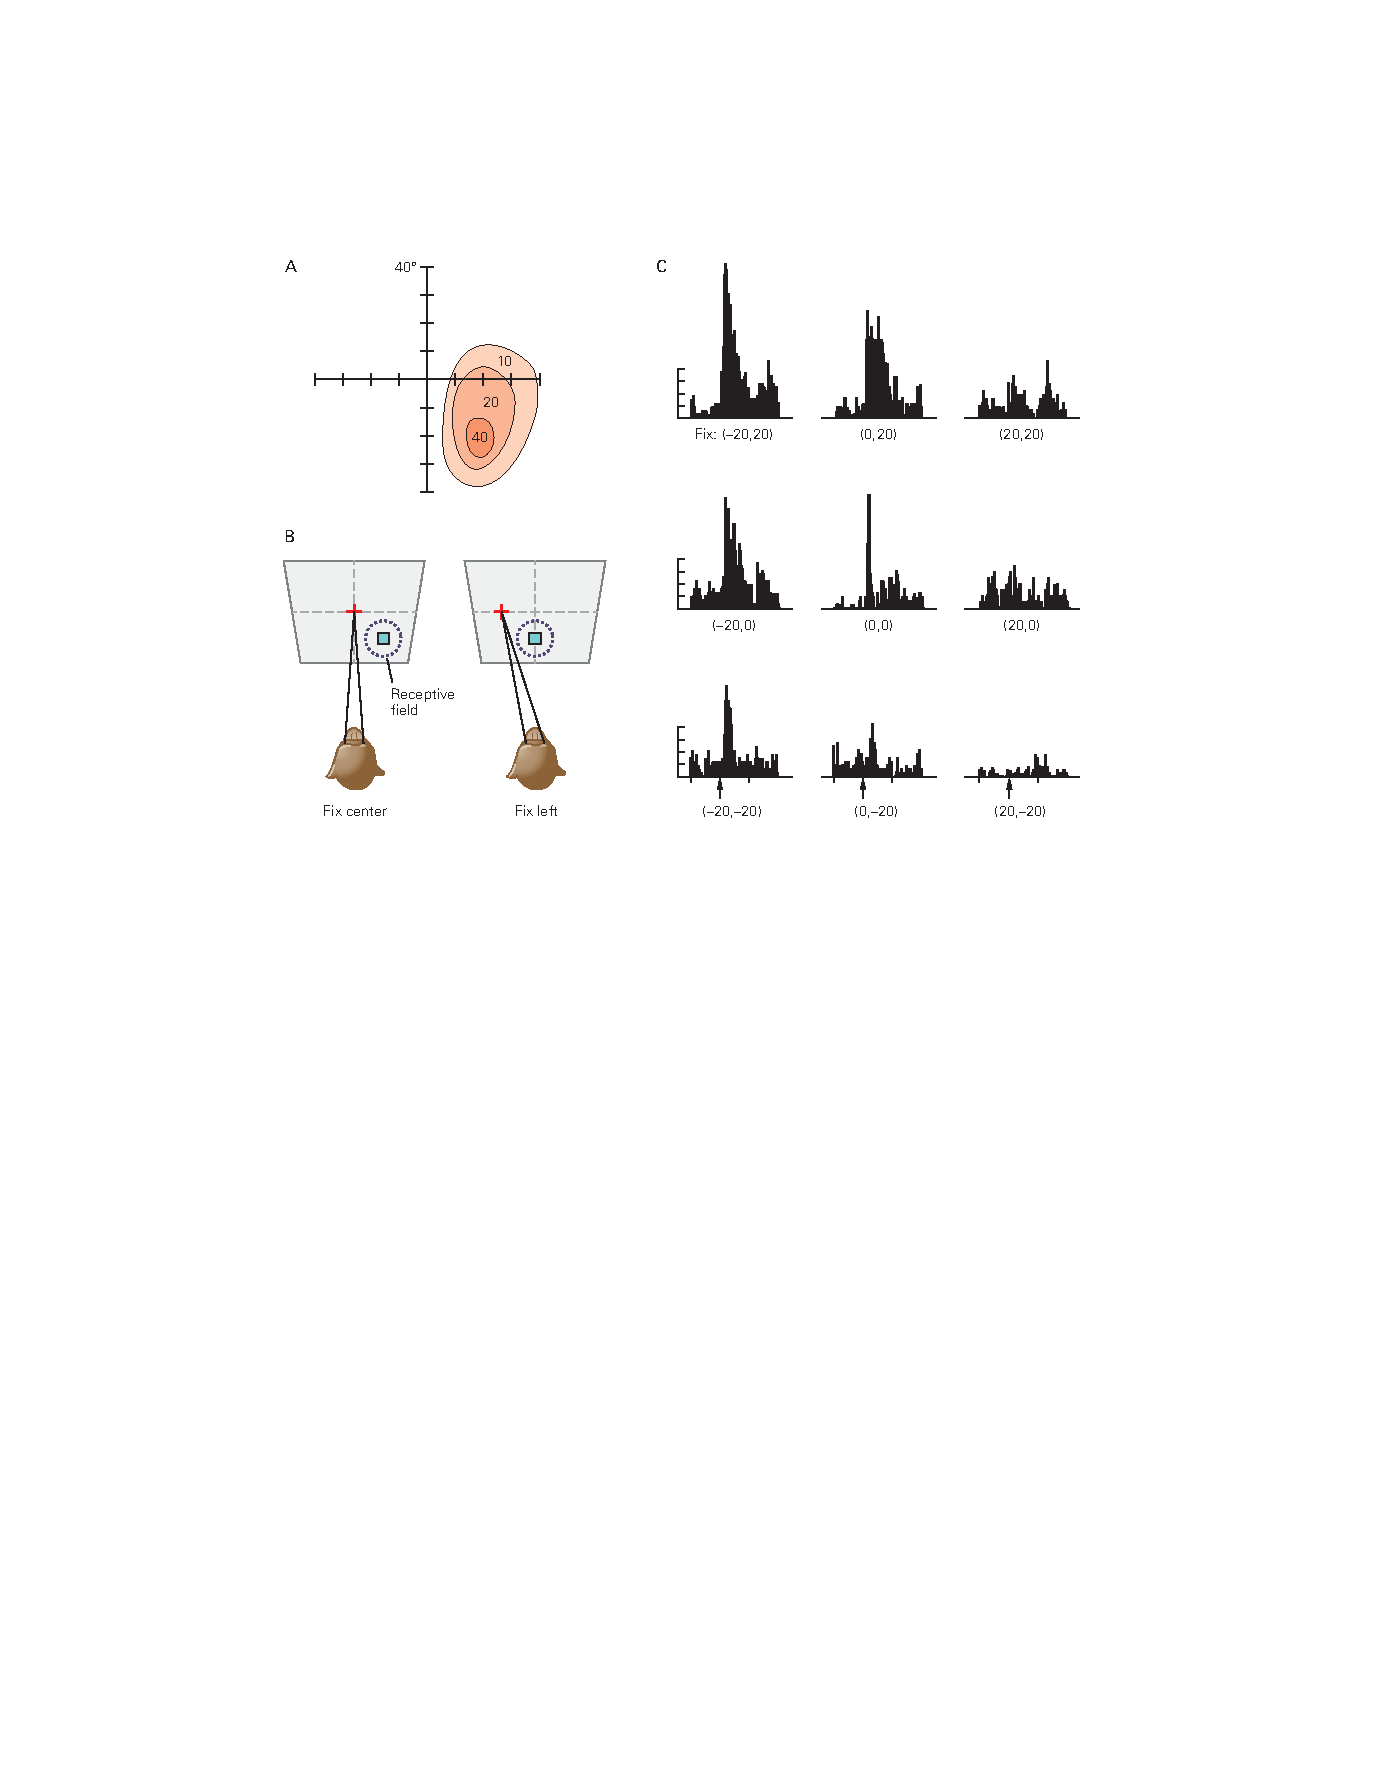
\includegraphics[width=0.7\linewidth]{chap25/fig_25_6}
	\caption{眼睛在眼眶中的位置会影响顶叶视觉神经元对视网膜感受野的反应。 A. 相对于中央凹的感受野。 等高线图表示不同空间位置的尖峰率。 数字是每个轮廓在最大位置的每秒峰值。 B.感受野随眼睛在空间移动。 在左边,猴子正在注视屏幕的中心。 在右侧,同一只猴子注视着中心左侧 20°。 对于 C 中的录音,刺激(蓝色方块)始终呈现在感受野的中心。 C. 在感受野的最佳位置对刺激的反应随着眼睛在眼眶中的位置而变化,从猴子注视-20°、20°的点时的最大值到猴子注视点时的最小值 在 20°,−20° 固定一个点。 箭头表示刺激闪光的开始。 试用时间,1.5秒; 纵坐标,25 个尖峰/格。 (经许可改编自 Andersen、Essick 和 Siegel 1985。版权所有 © 1985 AAAS。)}
	\label{fig:25_6}
\end{figure}


产生增益场的眼睛位置信号从何而来?
它可能来自眼睛位置的必然放电,也可能来自本体感受机制。
人眼肌肉有两种结构可能有助于动眼神经本体感觉:
肌梭和肌腱柱体,或栅栏末端,一种眼睛特有的结构。
区域 3a 是骨骼肌纺锤体投射到的体感皮层区域,代表眼睛的位置,由对侧眼眶的本体感受器产生(图 ~\ref{fig:25_7})。


\begin{figure}[htbp]
	\centering
	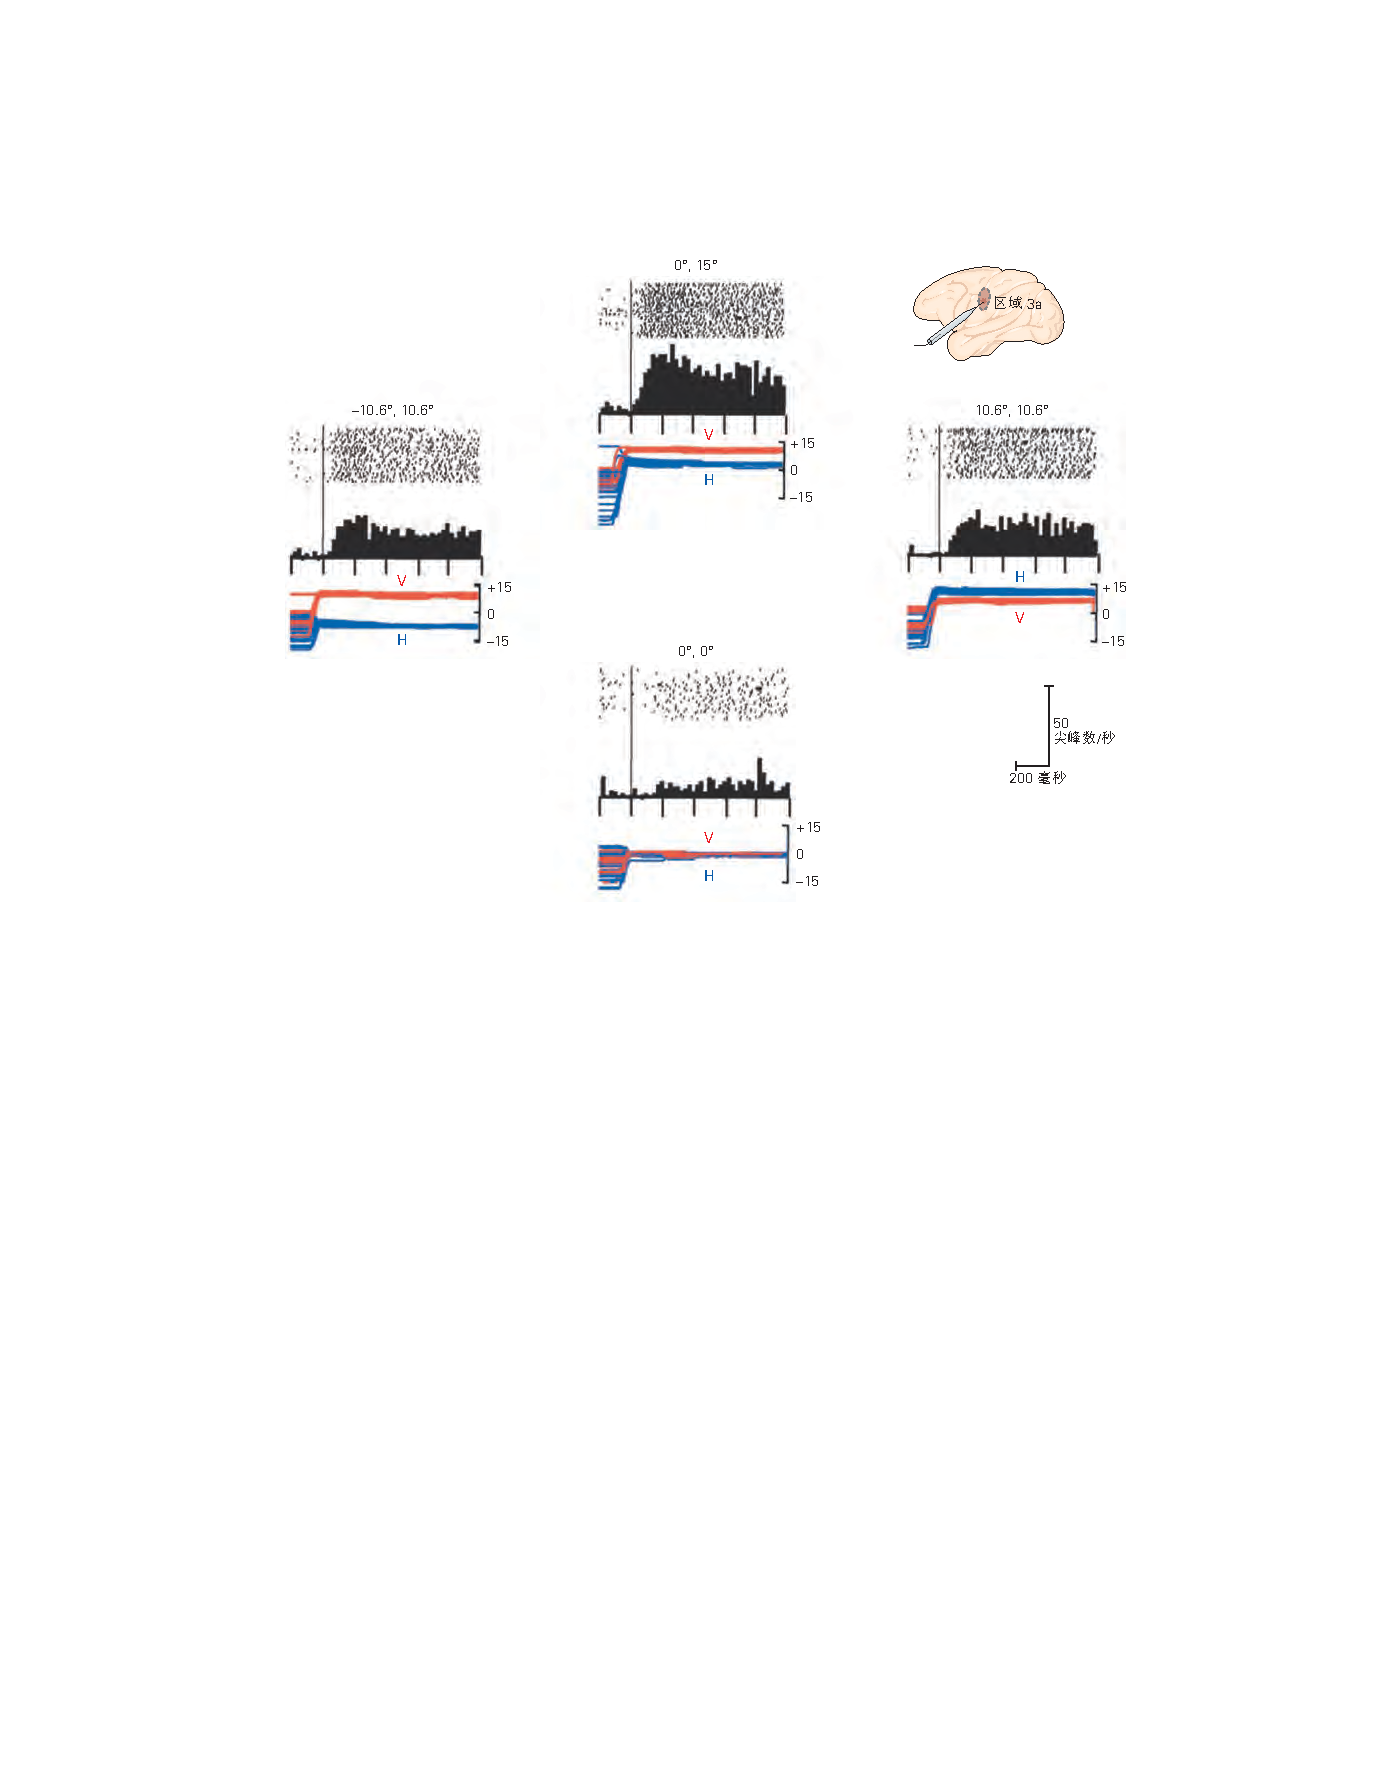
\includegraphics[width=0.8\linewidth]{chap25/fig_25_7}
	\caption{体感皮层区 3a 中的眼睛位置神经元。 每个面板显示水平 (H) 和垂直 (V) 眼睛位置以及猴子对每个光栅上方指示的眼睛位置进行扫视后神经元的活动。 当眼睛处于 0°、15° 时,神经元的反应比在 0°、0° 时要快得多。 (经许可转载自 Wang 等人,2007 年。)}
	\label{fig:25_7}
\end{figure}


然而,眼睛位置的本体感受测量滞后于眼睛位置的变化 60 毫秒,并且在扫视后的 150 毫秒内,增益场调节视觉反应,就好像猴子仍在看扫视前的目标一样,在推论放电已经很久之后 重新映射视觉响应。
因此,产生增益场的眼睛位置信号可能来自本体感受机制。
大脑有可能使用两种机制计算在眼球运动之前出现的物体的空间位置:
快速的推论放电和缓慢但比推论放电更准确的本体感受信号。
本体感受信号也可用于校准推论放电。



\section{视觉审查是由注意力和唤醒回路驱动的}

在 19 世纪,William James 将注意力描述为“头脑以清晰而生动的形式占据似乎同时可能出现的多个对象或思路中的一个。
它意味着从某些事情中退缩,以便有效地处理其他事情。” 
詹姆斯接着描述了两种不同的注意力:“它要么是被动的、反射性的、非自愿的、毫不费力的,要么是主动的、自愿的。
在被动的直接感官注意中,刺激是一种感官印象,要么非常强烈、大量,要么突然……大的东西、明亮的东西、移动的东西……血液。”


您在阅读本页时对本页的关注是自愿关注的一个例子。 如果一道亮光突然闪过,你的注意力可能会不由自主地从页面上移开。
在注意力焦点之外发生的视觉场景中的巨大变化通常会被忽略,直到主体将注意力转移到它们上,这种现象被称为变化失明(图~\ref{fig:25_8})。


\begin{figure}[htbp]
	\centering
	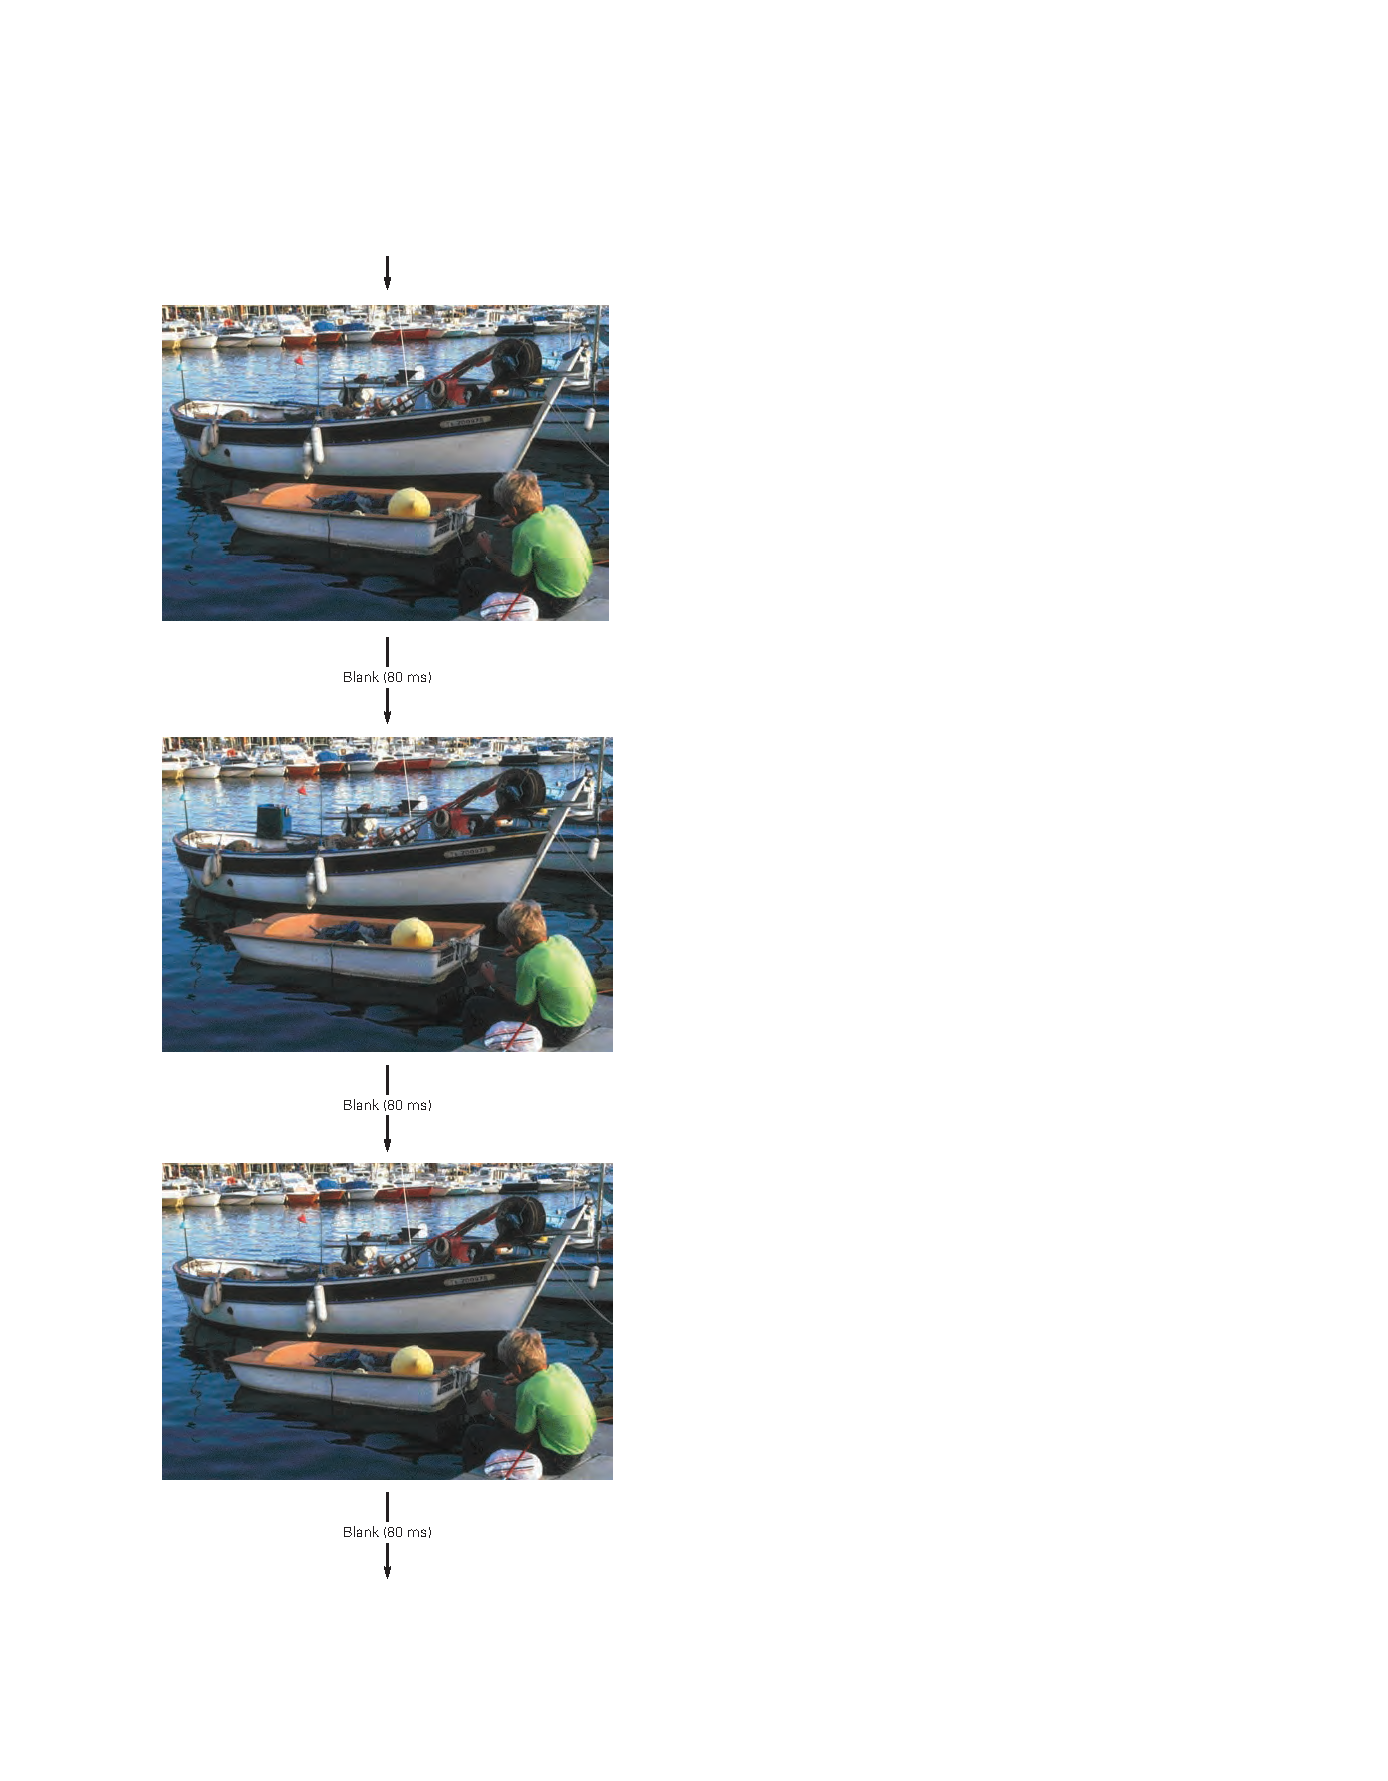
\includegraphics[width=0.5\linewidth]{chap25/fig_25_8}
	\caption{改变失明。 在变化失明测试中,先显示一张图片,然后是 80 毫秒的空白屏幕,然后是第二张图片,另一张空白屏幕,然后重复该循环(左)。 受试者被要求报告场景发生了什么变化。 尽管两张照片之间存在实质性差异,但大多数观察者需要多次重复才能发现差异。 (经许可转载自 Ronald Rensink。)}
	\label{fig:25_8}
\end{figure}


自愿注意与扫视眼球运动密切相关,因为中央凹的视锥细胞阵列比周边视网膜密集得多(第 ~\ref{chap:chap17}~章),并且将中央凹移至注意的对象允许进行比周边视觉可能进行的更细粒度的分析。 选择空间中的一个点的注意力,无论是否伴随眼跳,都称为空间注意力。
搜索特定类型的对象,例如红色和绿色 Q 中的红色 O,涉及第二种注意力,即特征注意力:在搜索中,你忽略绿色字母而只关注红色字母。


有意和无意的注意力会缩短反应时间并使视觉感知更加敏感。
这种提高的灵敏度包括以较低对比度检测物体并忽略靠近关注物体的干扰物的能力。
行为无关的提示(例如闪光)的突然出现,减少了对 300 毫秒后在同一位置出现的测试刺激的反应时间。
相反,当提示远离测试刺激出现时,反应时间会增加。
闪光会不自觉地引起人们对其位置的注意,从而加速对测试刺激的视觉反应。
类似地,当受试者计划对视野的特定部分进行扫视时,可以检测到任何物体的对比度阈值会通过提示提高 50\%。


临床研究长期以来一直将顶叶与视觉注意力联系起来。
右侧顶叶病变的患者视野正常。
当在简单的视觉环境中用单一刺激研究他们的视觉感知时,他们的反应是正常的。
然而,当呈现更复杂的视觉环境时,左右视觉半场都有物体,这些患者倾向于报告左半场(病变对侧)的内容少于右半场(病变同侧))。
这种缺陷,称为忽视(第~\ref{chap:chap59}~章),是因为注意力集中在病变同侧的视觉半场上。
即使患者只接受两种刺激,每个半视野一个,他们也报告说只看到同侧半视野的刺激。
当注意力集中在受影响的半野的一个刺激上,而第二个刺激出现在未受影响的半野时,患者没有能力将注意力转移到新的刺激上,即使从眼睛到纹状体和前纹状体皮质的感觉通路 完好无损。


这种对对侧视觉半视野的忽视延伸到对单个物体的对侧一半的忽视(图~\ref{fig:25_9})。
右顶叶缺损患者通常难以再现绘图。
例如,当被要求画一个时钟时,他们可能会将所有数字强制放在钟面的右侧,或者当被要求平分一条线时,他们可能会将中线放在该线实际中心的右侧。


\begin{figure}[htbp]
	\centering
	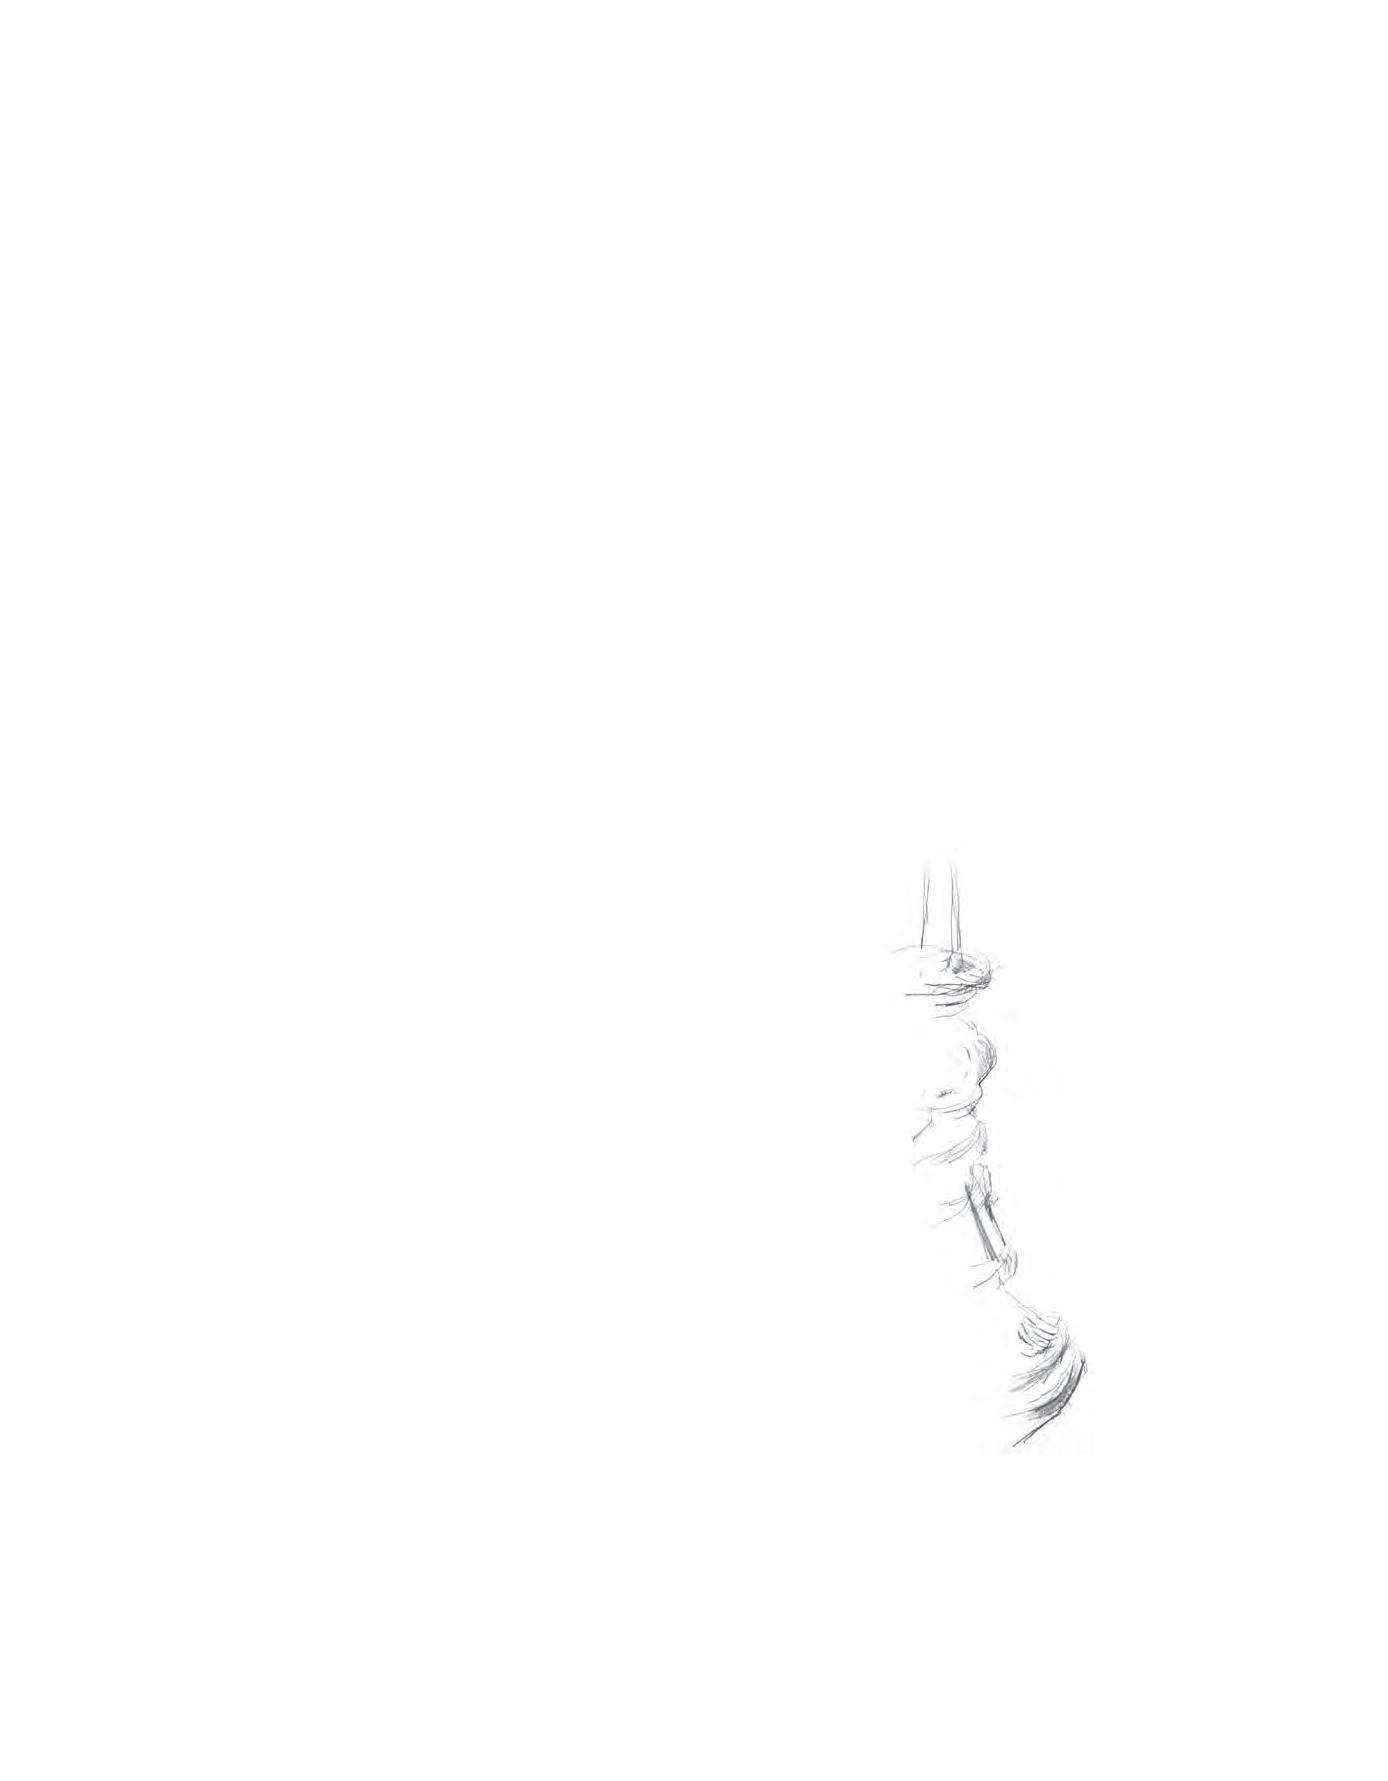
\includegraphics[width=0.5\linewidth]{chap25/fig_25_9}
	\caption{右顶叶损伤患者绘制的烛台图。病人忽略了烛台的左侧,只画了它的右半部分。(经许可转载自 Halligan 和 Marshall 2001。版权所有 © 2001 Academic Press。)}
	\label{fig:25_9}
\end{figure}


注意选择的过程在猴子的单个顶叶神经元水平上是显而易见的。
顶叶内外侧区域的神经元对视觉刺激的反应不仅取决于刺激的物理特性,还取决于它对猴子的重要性。
因此,对行为无关刺激的反应远小于对任何引起注意的事件的反应,例如在感受野中突然出现视觉刺激或计划对神经元的感受野进行扫视。


虽然外侧顶内区域的神经元共同代表整个视觉半场,但任何时刻活跃的神经元仅代表半场中的重要对象,即视野的优先图。
外侧顶叶内区域充当许多不同信号的汇合点:扫视规划、突然刺激发作和搜索特征的认知方面。


一个物体引起的神经元反应的绝对值本身并不能决定该动物是否正在注意该物体。
当一只猴子计划对视野中的刺激进行扫视时,注意力集中在扫视的目标上,而扫视计划引发的活动位于优先图的顶部。
然而,如果明亮的光线出现在视野的其他地方,注意力就会不由自主地被吸引到明亮的光线上,这会比扫视计划唤起更多的神经元活动。
因此,只能通过检查整个优先级图并选择其峰值来识别注意力点;
它不能仅通过监测任何一点的活动来识别(方框 25-1)。



\section{顶叶皮层为运动系统提供视觉信息}

视觉与辅助皮质和前运动皮质相互作用,为运动系统的动作做好准备。
例如,当你拿起一支铅笔时,你的手指与拇指的距离是铅笔的宽度;
当你拿起一杯饮料时,你的手指与拇指之间的距离与玻璃杯的宽度相同。
视觉系统有助于在您的手到达物体之前调整抓握宽度。
类似地,当您将一封信插入邮槽时,您的手会对齐以将信放入邮槽。
如果插槽倾斜,您的手也会倾斜以匹配。


顶叶皮层受损的患者不能仅使用视觉信息来调整他们的握持宽度或手腕角度,即使他们可以口头描述物体的大小或槽的方向。
相反,具有完整顶叶和腹侧流缺陷的患者无法描述物体的大小或其方向,但可以像正常受试者一样调整他们的抓握宽度和方向他们的手。
顶叶皮层中的神经元是操纵或移动物体所需信息的重要来源。
视觉引导运动背后的神经操作涉及识别目标、指定它们的品质,并最终生成运动程序来完成运动。
顶叶皮层中的神经元提供手指独立运动所需的视觉信息。


顶叶皮层中空间的表征不像初级视觉皮层中的视网膜专题图那样被组织成一个单一的图。
相反,它至少分为四个区域(LIP、MIP、VIP、AIP),以适合各个运动系统的方式分析视觉世界。
这四个区域将视觉信息投射到控制个体自主运动的前运动和额叶皮层区域(图 25-13)。


内侧顶内区域的神经元描述伸手可及的运动目标,并投射到控制伸手动作的运动前区。
前顶内皮层的神经元会发出可抓取物体的大小、深度和方向的信号。
该区域的神经元对可能成为抓取运动目标的刺激做出反应,并且当动物进行运动时,这些神经元也会活跃(图 25-14)。
外侧顶内区域的神经元指定眼跳的目标,并投射到额叶眼区。


因为猴子看不到它的嘴巴,腹侧顶内区有双峰神经元,它们对面部的触觉刺激(图 25-15)和视觉世界中接近触觉感受野的物体做出反应,使大脑能够估计 物体靠近嘴巴。
腹侧顶内区投射到运动前皮层的面部区域。




\section{要点}

1. 世界的图像通过眼睛进入大脑,眼睛在头部不断移动。
视觉系统必须补偿眼睛位置的变化,以根据视网膜位置计算空间位置。
Helmholtz 假设大脑通过将驱动眼睛的运动信号反馈到视觉系统来解决这个问题,以补偿眼球运动的影响。
这种对视觉系统的运动反馈称为推论放电。


2. 向动眼神经系统提供视觉信息的外侧顶内区域的神经元显示了这种必然放电的证据。
如果即将发生的眼跳将刺激带入其感受野,通常不会对空间中的特定刺激做出反应的神经元将对其做出反应。


3. 这种感受野重新映射取决于从上丘中间层到丘脑内侧背核再到额眼区的通路。
内侧背核失活会损害猴子在扫视后识别眼睛落在何处的能力,这表明必然放电具有感知和运动作用。


4. Sherrington 假设大脑使用眼睛位置根据物体图像在视网膜上的位置来计算物体的空间位置。
体感皮层中有眼睛位置的表示。
眼睛位置调节顶叶神经元的视觉反应,空间中的目标位置很容易从这种调节中计算出来。


5. 一个悬而未决的问题是大脑如何在眼睛位置和必然放电机制之间进行选择以确定空间位置。
因为必然放电先于眼睛位置的变化而本体感觉随之改变,所以大脑可以在不同时间使用这两种位置吗?


6. 注意力是大脑选择世界上的对象进行进一步分析的能力。
没有注意力,空间感知就会受到严重限制。
例如,人类很难注意到视觉世界的变化,除非他们的注意力被吸引到变化的空间位置。


7. 顶叶皮层神经元的活动预测了猴子的空间注意力,这是通过它们的感知阈值来衡量的。
顶叶皮层将许多不同的信号——运动信号、视觉信号、认知信号——相加,以创建视野的优先级图。
运动系统使用这张地图来选择运动目标。
视觉系统使用相同的地图来寻找视觉注意力的轨迹。


8. 顶叶皮层的损伤导致对侧视觉世界的忽视。


9. 顶叶皮层提供的视觉信息使运动系统能够在手实际落在目标上之前调整手的抓地力以匹配其到达的物体的大小。
相比之下,由于颞下皮层损伤导致知觉缺陷的患者可以很好地调整他们的抓握,即使他们无法完美地描述他们所触及的物体的性质或大小。


10. 顶内沟中至少有四种不同的视觉地图,每一种都对应于特定的运动工作区。


11. 顶内前区的神经元对抓取目标作出反应,即使猴子在完全黑暗中进行抓取动作时也会作出反应,并投射到运动前皮层的抓取区域。


12. 腹侧顶内区的神经元对靠近嘴巴的物体做出反应,在面部有触觉感受野,并投射到运动前皮层的嘴巴区域。 


13. 内侧顶内区域的神经元具有手臂位置的表征并对到达的目标做出反应。


14. 外侧顶内区域的神经元对眼球运动目标和视觉注意对象作出反应,在眼球运动前放电,并具有眼球位置的表征。
这些神经元的活动受眼睛在眼眶中的位置调节。


15. 体感皮层 3a 区面部区域的神经元具有眼球在由对侧眼产生的眼眶位置的表征。

